\section{논문 요약}{\label{sec:review}}

\subsection{Multi-modal fusion transformer for end-to-end autonomous driving}{\label{subsec:Transfuser}}
\begin{figure}[htp]
    \centering
    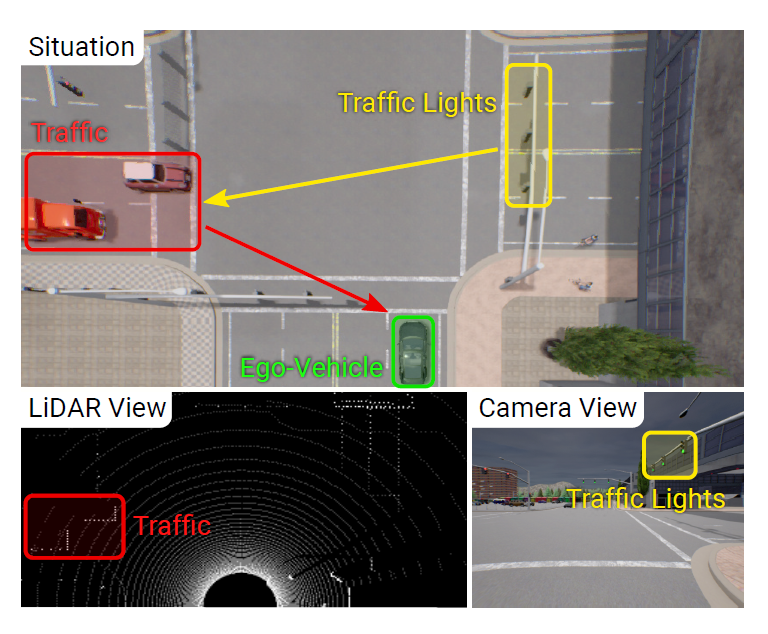
\includegraphics[width=0.8\textwidth]{figures/Transfuser_case.png}
    \caption{논문에서 해결하려는 문제 상황}
    \label{fig:tf_case}
\end{figure}
이 논문은 \autoref{fig:tf_case} 의 상황처럼
라이다(LiDAR : Light Detection And Ranging) 센서로 얻을 수 있는 주변의 차량의 위치에 따른 교통정보와
카메라로 얻을 수 있는 신호기에 따른 교통정보가 다른 경우,
두 센서로부터 얻을 수 있는 정보를 결합하여 차량의 주행을 제어하는 것을 목적으로 한다.
\begin{figure}[htp]
    \centering
    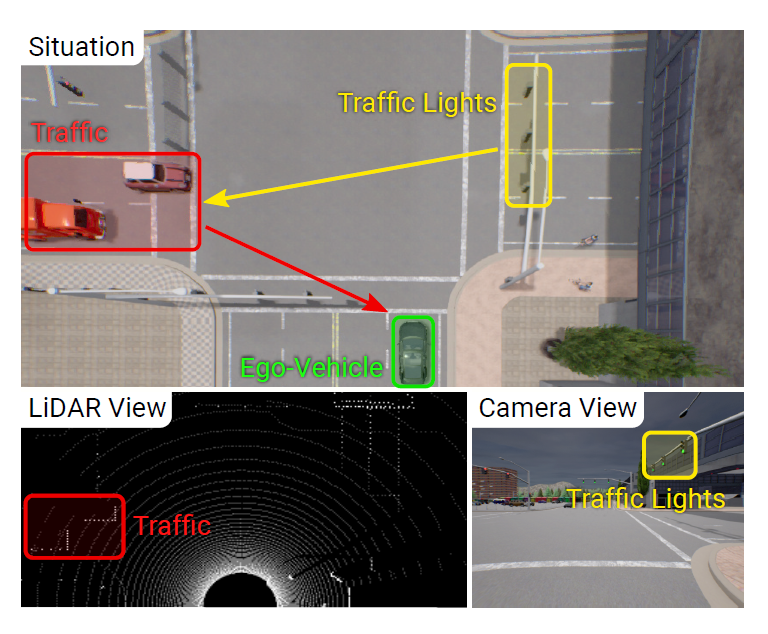
\includegraphics[width=\textwidth]{figures/Transfuser.png}
    \caption{Transfuser 구조}
    \label{fig:tf}
\end{figure}
\autoref{fig:tf}는 Transfuser의 구조를 보여준다.
두 센서의 출력으로부터 Resnet 구조\cite{Resnet}를 이용하여 정보를 추출하는 과정에서,
각 layer의 출력단으로부터 추출된 정보를 Transformer\cite{Transformer}를 이용하여 결합하는 것을 확인할 수 있다.

\subsubsection{method}{\label{subsubsec:tf_method}}
% 목적, 입력, 전처리, 출력, 학습, 평가
논문에서 제시한 \textbf{목표}는 시내 도로 주행에서의 point-to-point navigation이다.
point-to-point navigation은 차량이 목표지점까지
waypoint를 따라
교통법규를 지키면서
다른 차량과의 상호작용을 하며
완주하는 것을 의미한다.

이를 달성하기 위한 방법으로 강화학습 기법 중 하나인 Imitation Learning을 채용하였다.
Imitation Learning은 전문가가 직접 주행한 데이터를 따라하도록 agent의 policy를 학습하는 것을 의미한다.
\textbf{데이터셋}은 자율주행 오픈소스 시뮬레이터 CARLA\cite{CARLA}에 있는 urban 가상환경에서 수집했다.
데이터의 왜곡을 줄이기 위해 이미지 입력의 중앙을 잘라내어 256X256X3 크기로 사용했다.
LiDAR 센서의 출력 또한 주변부분의 정보를 기반으로 256X256X2 사이즈로 잘라내어 사용하였다.
채널의 한쪽은 지면 위, 한쪽은 지면 아래를 의미한다.
\textbf{출력}은 PID controller로 차량을 제어하기 위해 4개의 waypoint $\{w_t = (x_t, y_t)\}_{t=1}^T$ 로 설정했다.



\subsection{YOLOv7: Trainable bag-of-freebies sets new state-of-the-art for real-time object detectors}{\label{subsec:yolov7}}

asdf